\documentclass[]{book}
\usepackage{lmodern}
\usepackage{amssymb,amsmath}
\usepackage{ifxetex,ifluatex}
\usepackage{fixltx2e} % provides \textsubscript
\ifnum 0\ifxetex 1\fi\ifluatex 1\fi=0 % if pdftex
  \usepackage[T1]{fontenc}
  \usepackage[utf8]{inputenc}
\else % if luatex or xelatex
  \ifxetex
    \usepackage{mathspec}
  \else
    \usepackage{fontspec}
  \fi
  \defaultfontfeatures{Ligatures=TeX,Scale=MatchLowercase}
  \newcommand{\euro}{€}
\fi
% use upquote if available, for straight quotes in verbatim environments
\IfFileExists{upquote.sty}{\usepackage{upquote}}{}
% use microtype if available
\IfFileExists{microtype.sty}{%
\usepackage{microtype}
\UseMicrotypeSet[protrusion]{basicmath} % disable protrusion for tt fonts
}{}
\usepackage[margin=1in]{geometry}
\usepackage{hyperref}
\PassOptionsToPackage{usenames,dvipsnames}{color} % color is loaded by hyperref
\hypersetup{unicode=true,
            pdftitle={POLS 503: Advanced Quantitative Political Methodology: The Notes},
            pdfauthor={Jeffrey B. Arnold},
            pdfborder={0 0 0},
            breaklinks=true}
\urlstyle{same}  % don't use monospace font for urls
\usepackage{longtable,booktabs}
\usepackage{graphicx,grffile}
\makeatletter
\def\maxwidth{\ifdim\Gin@nat@width>\linewidth\linewidth\else\Gin@nat@width\fi}
\def\maxheight{\ifdim\Gin@nat@height>\textheight\textheight\else\Gin@nat@height\fi}
\makeatother
% Scale images if necessary, so that they will not overflow the page
% margins by default, and it is still possible to overwrite the defaults
% using explicit options in \includegraphics[width, height, ...]{}
\setkeys{Gin}{width=\maxwidth,height=\maxheight,keepaspectratio}
\setlength{\parindent}{0pt}
\setlength{\parskip}{6pt plus 2pt minus 1pt}
\setlength{\emergencystretch}{3em}  % prevent overfull lines
\providecommand{\tightlist}{%
  \setlength{\itemsep}{0pt}\setlength{\parskip}{0pt}}
\setcounter{secnumdepth}{5}

%%% Use protect on footnotes to avoid problems with footnotes in titles
\let\rmarkdownfootnote\footnote%
\def\footnote{\protect\rmarkdownfootnote}

%%% Change title format to be more compact
\usepackage{titling}

% Create subtitle command for use in maketitle
\newcommand{\subtitle}[1]{
  \posttitle{
    \begin{center}\large#1\end{center}
    }
}

\setlength{\droptitle}{-2em}
  \title{POLS 503: Advanced Quantitative Political Methodology: The Notes}
  \pretitle{\vspace{\droptitle}\centering\huge}
  \posttitle{\par}
  \author{Jeffrey B. Arnold}
  \preauthor{\centering\large\emph}
  \postauthor{\par}
  \predate{\centering\large\emph}
  \postdate{\par}
  \date{2016-04-19}


\usepackage{booktabs}

\DeclareMathOperator{\E}{E}
\DeclareMathOperator{\mean}{mean}
\DeclareMathOperator{\Var}{Var}
\DeclareMathOperator{\Cov}{Cov}
\DeclareMathOperator{\Cor}{Cor}
\DeclareMathOperator{\Bias}{Bias}
\DeclareMathOperator{\MSE}{MSE}
\DeclareMathOperator{\sd}{sd}
\DeclareMathOperator{\se}{se}
\DeclareMathOperator{\rank}{rank}
\DeclareMathOperator*{\argmin}{arg\,min}
\DeclareMathOperator*{\argmax}{arg\,max}

\newcommand{\mat}[1]{\boldsymbol{#1}}
\renewcommand{\vec}[1]{\boldsymbol{#1}}
\renewcommand{\T}{'}

\newcommand{\distr}[1]{\mathcal{#1}}
\newcommand{\dnorm}{\distr{N}}
\newcommand{\dmvnorm}[1]{\distr{N}_{#1}}

% Redefines (sub)paragraphs to behave more like sections
\ifx\paragraph\undefined\else
\let\oldparagraph\paragraph
\renewcommand{\paragraph}[1]{\oldparagraph{#1}\mbox{}}
\fi
\ifx\subparagraph\undefined\else
\let\oldsubparagraph\subparagraph
\renewcommand{\subparagraph}[1]{\oldsubparagraph{#1}\mbox{}}
\fi

\begin{document}
\maketitle

{
\setcounter{tocdepth}{1}
\tableofcontents
}
\chapter{Introduction}\label{introduction}

hello, world!

\chapter{Linear Regression and the Ordinary Least Squares (OLS)
Estimator}\label{linear-regression-and-the-ordinary-least-squares-ols-estimator}

Since we will largely be concerned with using linear regression for
inference, we will start by discussion the population parameter of
interest (population linear regression function), then the sample
statistic (sample linear regression function) and estimator (ordinary
least squares).

We will then consider the properties of the OLS estimator.

\section{Linear Regression Function}\label{linear-regression-function}

The \textbf{population linear regression function} is \[
r(x) = \E[Y | X = x] = \beta_0 + \sum_{k = 1}^{K} \beta_{k} x_k .
\] The population linear regression function is defined for random
variables, and will be the object to be estimated.

Names for \(\vec{y}\)

\begin{itemize}
\tightlist
\item
  dependent variable
\item
  explained variable
\item
  response variable
\item
  predicted variable
\item
  regressand
\item
  outcome variable
\end{itemize}

Names for \(\mat{X}\),

\begin{itemize}
\tightlist
\item
  indpendent variables
\item
  explanatory varaibles
\item
  treatment and control variables
\item
  predictor variables
\item
  covariates
\item
  regressors
\end{itemize}

To estimate the unkonwn population linear regression, we will use the
\textbf{sample linear regression function}, \[
\hat{r}(x_i) = \hat{y}_i = \hat\beta_0 + \sum_{k = 1}^{K} \hat\beta_{k} x_k .
\] However, we

\(\hat{Y}_i\) are the fitted or predicted value The \textbf{residuals}
or \textbf{errors} are the prediction errors of the estimates \[
\hat{\epsilon}_i = y_i - \hat{y}_i
\]

\(\vec{\beta}\) are the parameters; \(\beta_0\) is called the
\emph{intercept}, and \(\beta_{1}, \dots, \beta_{K}\) are called the
\emph{slope parameters}, or \emph{coefficients}.

The linear regression function can be written as a scalar function for
each observation, \(i = 1, \dots, N\), \[
\begin{aligned}[t]
y_i &= \beta_0 + \beta_1 x_{1,i} + \beta_2 x_{2,i} + \cdots + \beta_{K,i} + \varepsilon_i \\
 &= \beta_0 + \sum_{k = 1}^{K} \beta_k x_{k,i} + \varepsilon_i \\
&= \sum_{k = 0}^{K} \beta_k x_{k,i} + \varepsilon_i
\end{aligned}
\] where \(x_{0,i} = 1\) for all \(i \in 1:N\).

The linear regression can be more compactly written in matrix form, \[
\begin{aligned}[t]
  \begin{bmatrix}
    y_1 \\
    y_2 \\
    \vdots \\
    y_N
  \end{bmatrix} &=
  \begin{bmatrix}
    1 & x_{1,1} & x_{2,1} & \cdots & x_{K,1} \\
    1 & x_{1,2} & x_{2,2} & \cdots & x_{K,2} \\
    \vdots & \vdots & \vdots & \ddots & \vdots \\
    1 & x_{1,N}& x_{2,n} & \cdots & x_{K,N}
  \end{bmatrix}
  \begin{bmatrix}
    \beta_0 \\
    \beta_1 \\
    \beta_2 \\
    \vdots \\
    \beta_K
    \end{bmatrix}
  +
  \begin{bmatrix}
    \varepsilon_1 \\
    \varepsilon_2 \\
    \vdots \\
    \varepsilon_N
  \end{bmatrix}
\end{aligned} .
\] More compactly, the linear regression model can be written as, \[
\begin{aligned}[t]
  \underbrace{\vec{y}}_{N \times 1} &=
  \underbrace{\mat{X}}_{N \times K} \,\,
  \underbrace{\vec{\beta}}_{K \times 1} +
  \underbrace{\vec{\varepsilon}}_{N \times 1} .
\end{aligned}
\] The matrix \(\mat{X}\) is called the \emph{design} matrix. Its rows
are each observation in the data. Its columns are the intercept, a
column vector of 1's, and the values of each predictor.

\section{Ordinary Least Squares}\label{ordinary-least-squares}

Ordinary least squares (OLS) is an estimator of the slope and statistic
of the regression line\footnote{Ordinary least squares is distinguished
  from \emph{generalized least squares} (GLS).}. OLS finds values of the
intercept and slope coefficients by minimizing the squared errors, \[
\hat{\beta}_0, \hat{\beta}_1, \dots, \hat{\beta}_K
=
\argmin_{b_0, b_1, \dots, b_k} \sum_{i = 1}^{N}  \underbrace{{\left(y_i - b_0 - \sum_{k = 1}^{K} b_k x_{i,k} \right)}^2}_{\text{squared error}},
\] or, in matrix notation, \[
\begin{aligned}[t]
\hat{\vec{\beta}} &= \argmin_{\vec{b}} \sum_{i = 1}^N (y_i - \vec{b}\T \vec{x}_i)^2 \\
&= \argmin_{\vec{b}} \sum_{i = 1}^N u_i^2 \\
&= \argmin_{\vec{b}} \vec{u}' \vec{u}
\end{aligned}
\] where \(\vec{u} = \vec{y} - \mat{X} \vec{\beta}\).

In most statistical models, including even genalized linear models such
as logit, the solution to this minimization problem would be solved with
optimization methods that require interation. One nice feature of OLS is
that there is a closed form solution for \(\hat{\beta}\) even in the
multiple regression case, so no iterative optimization methods need to
be used.

In the bivariate regression case, the OLS estimators for \(\beta_0\) and
\(\beta_1\) are \[
\begin{aligned}[t]
\hat{\beta}_0 &= \bar{y} - \hat\beta_1 \bar{x} \\
\hat{\beta}_1 7= \frac{\sum_{i = 1}^N (x_i - \bar{x}) (y_i - \bar{y})}{\sum_{i = 1}^N (x_i - \bar{x})^2} \\
&= \frac{\Cov(\vec{x} \vec{y})}{\Var{\vec{x}}}
&= \frac{\text{Sample covariance betweeen $\vec{x}$ and $\vec{y}$}}{\text{Sample variance of $\vec{x}$}} .
\end{aligned}
\] In the multiple regression case, the OLS estimator for
\(\hat{\vec{\beta}}\) is \[
\hat{\vec{\beta}} = \left( \mat{X}' \mat{X} \right)^{-1} \mat{X}' \vec{y} .
\] The term \(\mat{X}' \mat{X}\) is similar to the variance of
\(\vec{x}\) in the bivariate case. The term \(\mat{X}' \vec{y}\) is
similar to the covariance between \(\mat{X}\) and \(\vec{y}\) in the
bivariate case.

The sample linear regression function estimated by OLS has the following
properties:

\begin{enumerate}
\def\labelenumi{\arabic{enumi}.}
\tightlist
\item
  Residuals sum to zero, \[
  \sum_{i = 1}^N \hat{\epsilon}_i = 0 .
  \] This implies that the mean of residuals is also 0.
\item
  The regression function passes through the point
  \((\bar{\vec{y}}, \bar{\vec{x}}_1, \dots, \bar{\vec{x}_K})\). In other
  words, the following is always true, \[
  \bar{\vec{y}} = \hat\beta_0 + \sum_{k = 1}^K \hat\beta_k \bar{\vec{x}}_k .
  \]
\item
  The resisuals are uncorrelated with the predictor \[
  \sum_{i = 1}^N x_i \hat{\epsilon}_i = 0
  \]
\item
  The residuals are uncorrelated with the fitted values \[
  \sum_{i = 1}^N \hat{y}_i \hat{\varepsilon}_i = 0
  \]
\end{enumerate}

\section{Properties of the OLS
Estimator}\label{properties-of-the-ols-estimator}

\subsection{What makes an estimator
good?}\label{what-makes-an-estimator-good}

Estimators are evaluated not on how close an estimate in a given sample
is to the population, but how their sampling distributions compare to
the population. In other words, judge the \emph{methodology}
(estimator), not the \emph{result}
(estimate).{[}\^{}ols-properties-references{]}

Let \(\theta\) be the population parameter, and \(\hat\theta\) be an
estimator of that population parameter.

\begin{description}
\item[Bias]
The bias of an estimator is the difference between the mean of its
sampling distribution and the population parameter,
\[\Bias(\hat\theta) = \E(\hat\theta) - \theta .\]
\item[Variance]
The variance of the estimator is the variance of its sampling
distribution, \(\Var(\theta)\).
\item[Efficiency (Mean squared error)]
An efficient estimator is one that minimizes a given ``loss function'',
which is a penalty for missing the population average. The most common
loss function is squared loss, which gives the \emph{Mean Squared Error
(MSE)} of an estimator.

\[\MSE(\hat\theta) = \E\left[{(\hat\theta - \theta)}^{2}\right] =  (\E(\hat\theta) - \theta)^2 + \E(\hat\theta - \E(\hat\theta))^2 = \Bias(\hat\theta)^2 + \Var(\hat\theta)\]

The mean squared error is a function of both the bias and variance of an
estimator.

This means that some biased estimators can be more efficient : than
unbiased estimators if their variance offsets their bias.\footnote{It
  follows from the definition of MSE, that biased estimator,
  \(\hat\theta_{B}\), has a lower MSE than an unbiased estimator,
  \(\hat\theta_{U}\), if
  \(\Bias(\theta_B)^2 < \Var(\theta_U) - \Var(\theta_B)\).}
\end{description}

\textbackslash{}begin\{table\}

\textbackslash{}caption\{\label{tab:unnamed-chunk-1}Examples of clocks as
``estimators'' of the time\footnote{Example from
  \href{http://faculty.washington.edu/cadolph/503/topic3.pw.pdf}{Chris
  Adolph}}\} \centering

\begin{tabular}[t]{l|l|l}
\hline
  & Biased & Variance\\
\hline
Stopped clock & Yes & High\\
\hline
Random clock & No & High\\
\hline
Clock that is "a lot " fast & Yes & Low\\
\hline
Clock that is "a little" fast & Yes & Low\\
\hline
Atomic clock & No & Low\\
\hline
\end{tabular}

\textbackslash{}end\{table\}

Another property is \textbf{consistency}. Consistency is an asymptotic
property\footnote{As the number of observations goes to infinity.}, that
roughly states that an estimator converges to the truth as the number of
obserservations grows, \(\E(\hat\theta - \theta) \to 0\) as
\(N \to \infty\). Roughly, this means that if you had enough (infinite)
data, the estimator will give you the true value of the parameter.

\subsection{Properties of OLS}\label{properties-of-ols}

\begin{itemize}
\tightlist
\item
  When is OLS unbiased?
\item
  When is OLS consistent?
\item
  When is OLS efficient?
\end{itemize}

\begin{enumerate}
\def\labelenumi{\arabic{enumi}.}
\item
  \textbf{Linearity} The popluation model is \[
     \vec{y} = \mat{X} \vec{\beta} + \vec{\varepsilon}
     \] where \(\vec{\varepsilon}\) is an unobserved random error or
  disturbance term with \(\E(\varepsilon) = 0\).
\item
  Random/iid sample. \((y_i, \vec{x}_i')\) are a random sample from the
  population.
\item
  \textbf{No Perfect Collinearity}. There is no exact \emph{linear}
  relationships among the independent variables. \(\mat{X}\) is a
  \(N \times K\) matrix with rank \(K\).
\item
  Zero conditional mean. The error, \(\varepsilon\), has an expected
  value of zero, conditional on the predictors. \[
  \E(\varepsilon | X) = 0
  \]
\item
  Constant variance (Homoskedasticity). The error has the same variance
  conditional on the predictors, for all observations, \[
  \E(\epsilon_i | \vec{x}_i) = \sigma^2) \text{ for all $i$}
  \]
\item
  Fixed \(\mat{X}\) or \(\mat{X}\) measured without error and
  independent of the error.
\item
  Normal disturbances: \(\epsilon_i|\mat{X} \sim N(0, \sigma^2)\).
\end{enumerate}

What do these assumptions give us?

\begin{itemize}
\tightlist
\item
  Identification of OLS: Under Assumption 1, OLS can be estimated. In
  other words, there is a \emph{unique} \(\hat\beta\) that minimizes the
  sum of squared errors.
\item
  Unbiasedness of OLS: Under Assumptions 1--4, OLS is unbiased. \[
  \E(\hat{\vec{\beta}}) = \vec{\beta}
  \]
\item
  Gauss-Markov theorem. Under Assumptions 1--5, OLS is the best linear
  unbiased estimator of \(\vec{\beta}\). \emph{Linear} means that the
  estimates can be written as a linear functions of the outcomes, \[
    \tilde{\beta}_j = \sum_{i = 1}^n w_{i,j} y_i
    \] \emph{Best} means that it has the smallest variance. This means
  for any unbiased and linear estimator, \(\tilde{\beta}\), the OLS
  estimator, \(\hat{\beta}_{OLS}\), has a smaller variance, \[
    \Var(\tilde{\beta}) > \Var(\hat{\beta}_{OLS})
    \] Not that this does not imply that OLS has the lowest MSE of any
  estimator, since a biased estimator could have a lower MSE. In fact,
  for any regression with three or more variables, there is a ridge
  estimator with a lower MSE.
\end{itemize}

\begin{longtable}[c]{@{}lll@{}}
\toprule
\begin{minipage}[b]{0.27\columnwidth}\raggedright\strut
Assumption
\strut\end{minipage} &
\begin{minipage}[b]{0.27\columnwidth}\raggedright\strut
Formal statement
\strut\end{minipage} &
\begin{minipage}[b]{0.32\columnwidth}\raggedright\strut
Consequence of violation
\strut\end{minipage}\tabularnewline
\midrule
\endhead
\begin{minipage}[t]{0.27\columnwidth}\raggedright\strut
No (perfect) collinearity
\strut\end{minipage} &
\begin{minipage}[t]{0.27\columnwidth}\raggedright\strut
\(\rank(\mat{X}) = K, K < N\)
\strut\end{minipage} &
\begin{minipage}[t]{0.32\columnwidth}\raggedright\strut
Coefficients unidentified
\strut\end{minipage}\tabularnewline
\begin{minipage}[t]{0.27\columnwidth}\raggedright\strut
\(\mat{X}\) is exogenous
\strut\end{minipage} &
\begin{minipage}[t]{0.27\columnwidth}\raggedright\strut
\(\E(\mat{X} \vec{\varepsilon}) = 0\)
\strut\end{minipage} &
\begin{minipage}[t]{0.32\columnwidth}\raggedright\strut
Biased, even as \(N \to \infty\)
\strut\end{minipage}\tabularnewline
\begin{minipage}[t]{0.27\columnwidth}\raggedright\strut
Disturbances have mean 0
\strut\end{minipage} &
\begin{minipage}[t]{0.27\columnwidth}\raggedright\strut
\(\E(\varepsilon) = 0\)
\strut\end{minipage} &
\begin{minipage}[t]{0.32\columnwidth}\raggedright\strut
Biased, even as \(N \to \infty\)
\strut\end{minipage}\tabularnewline
\begin{minipage}[t]{0.27\columnwidth}\raggedright\strut
No serial correlation
\strut\end{minipage} &
\begin{minipage}[t]{0.27\columnwidth}\raggedright\strut
\(\E(\varepsilon_i \varepsilon_j) = 0\), \(i \neq j\)
\strut\end{minipage} &
\begin{minipage}[t]{0.32\columnwidth}\raggedright\strut
Unbiased, wrong se
\strut\end{minipage}\tabularnewline
\begin{minipage}[t]{0.27\columnwidth}\raggedright\strut
Homoskedastic errors
\strut\end{minipage} &
\begin{minipage}[t]{0.27\columnwidth}\raggedright\strut
\(\E(\vec{\varepsilon}\T \vec{\varepsilon})\)
\strut\end{minipage} &
\begin{minipage}[t]{0.32\columnwidth}\raggedright\strut
Unbiased, wrong se
\strut\end{minipage}\tabularnewline
\begin{minipage}[t]{0.27\columnwidth}\raggedright\strut
Gaussian errors
\strut\end{minipage} &
\begin{minipage}[t]{0.27\columnwidth}\raggedright\strut
\(\varepsilon \sim \dnorm(0, \sigma^2)\)
\strut\end{minipage} &
\begin{minipage}[t]{0.32\columnwidth}\raggedright\strut
Unbiased, se wrong unless \(N \to \infty\)
\strut\end{minipage}\tabularnewline
\bottomrule
\end{longtable}

Note that these assumptions can be sometimes be written in largely
equivalent, but slightly different forms.

\section{References}\label{references}

\begin{itemize}
\tightlist
\item
  Wooldrige, Ch 3.
\item
  Fox, Ch 6, 9.
\end{itemize}

\chapter{OLS Troubleshooting and
Diagnostics}\label{ols-troubleshooting-and-diagnostics}

\section{Multi-Collinearity}\label{multi-collinearity}

\section{Omitted Variable Bias}\label{omitted-variable-bias}

\section{Measurement Error}\label{measurement-error}

\section{Non-linearity}\label{non-linearity}

\section{Heteroskedasticity and
Auto-correlation}\label{heteroskedasticity-and-auto-correlation}

Note, that OLS assumes that the variance of the the disturbances is
constant \(\hat{Y} - Y = \varepsilon = \sigma^2\). What happens if it
isn't?

\[
\mat{\Sigma} =
\begin{bmatrix}
\Var(\varepsilon_1) & \Cov(\varepsilon_1, \varepsilon_2) & \cdots & \Cov(\varepsilon_1, \varepsilon_N) \\
\Var(\varepsilon_2, \varepsilon_1) & \Var(\varepsilon_2) & \cdots & \Cov(\varepsilon_2, \varepsilon_N) \\
\vdots & \vdots & \ddots & \vdots \\
\Cov(\varepsilon_N, \varepsilon_1) & \Cov(\varepsilon_N, \varepsilon_2) & \cdots & \Cov(\varepsilon_N) \\
\end{bmatrix} \\
\Sigma =
\begin{bmatrix}
\E(\varepsilon_1^2) & \E(\varepsilon_1 \varepsilon_2) & \cdots & \E(\varepsilon_1 \varepsilon_N) \\
\E(\varepsilon_2 \varepsilon_1) & \E(\varepsilon_2^2) & \cdots & \E(\varepsilon_2 \varepsilon_N) \\
\vdots & \vdots & \ddots & \vdots \\
\E(\varepsilon_N \varepsilon_1) & \E(\varepsilon_N \varepsilon_2) & \cdots & \E(\varepsilon_N^2) \\
\end{bmatrix} \\
\] The matrix can be written more compactly as, \[
\mat{\Sigma} = \E(\vec{\varepsilon} \vec{\varepsilon}\T)
\]

An assumption is that errors are independent,
\(\E(\epsilon_i \epsilon_j)\) for all \(i \neq j\). This means that all
off-diagonal elements of \(\mat{\Sigma}\) are 0\$. Additionally, all
\(\epsilon_i\) are assumed to have the same variance, \(\sigma^2\).
Thus, the variance-covariance matrix of the errors is a assumed to have
a diagonal matrix with the form, \[
\mat{\Sigma} = 
\begin{bmatrix}
\sigma^2 & 0 & \cdots & 0 \\
0 & \sigma^2 & \cdots & 0 \\
\vdots & \vdots & \ddots & \vdots \\
0 & 0 & \cdots & \sigma^2
\end{bmatrix} 
= \sigma^2 \mat{I}_N
\] If these assumptions of the errors do not hold, then \(\Sigma\) does
not take this form, and more complicated models than OLS need to be used
to get correct standard errors.

\section{Non-constant variance
(Heteroskedasticity)}\label{non-constant-variance-heteroskedasticity}

The homoskedastic case assumes that each eror term has its own variance.
In the heteroskedastic case, each distrurbance may have its own
variance, but they are still uncorrelated (\(\mat{\Sigma}\) is diagonal)
\[
\mat{\Sigma} = 
\begin{bmatrix}
\sigma_1^2 & 0 & \cdots & 0 \\
0 & \sigma_2^2 & \cdots & 0 \\
\vdots & \vdots & \ddots & \vdots \\
0 & 0 & \cdots & \sigma_N^2
\end{bmatrix}
\] The problem is that now there are \(N\) variance parameters to
estimate, in addition to the \(K\) slope coefficients. Now, there are
more parameters than we can estimate. With heteroskedasticity, OLS with
be unbiased, but the standard errors will be incorrect.

More general case allows for heteroskedasticity, and autocorrelation
(\(\Cov(\varepsilon_i, \varepsilon_j) \neq 0\)), \[
\mat{\Sigma} = 
\begin{bmatrix}
\sigma_1^2 & \sigma_{1,2} & \cdots & \sigma_{1,N} \\
\sigma_{2,1} & \sigma_2^2 & \cdots & \sigma_{2,N} \\
\vdots & \vdots & \ddots & \vdots \\
\sigma_{N,1} & \sigma_{N,2} & \cdots & \sigma_N^2
\end{bmatrix} 
\] As with heteroskedasticity, OLS with be unbiased, but the standard
errors will be incorrect.

\chapter{Appendix}\label{appendix}

\section{Multivariate Normal
Distribution}\label{multivariate-normal-distribution}

The multivariate normal distribution is the generalization of the
univariate normal distribution to more than one dimension.\footnote{See
  \href{https://en.wikipedia.org/wiki/Multivariate_normal_distribution}{Multivariate
  normal distribution} and references therein.} The random variable,
\(\vec{x}\), is a length \(k\) vector. The \(k\) length vector
\(\vec{\mu}\) are the means of \(\vec{x}\), and the \(k \times k\)
matrix, \(\mat{\Sigma}\), is the variance-covariance matrix, \[
\begin{aligned}[t]
\vec{x} &\sim \dmvnorm{k}\left(\vec{\mu}, \mat{\Sigma} \right) \\
\begin{bmatrix}
x_1 \\
x_2 \\
\vdots \\
x_k
\end{bmatrix}
& \sim
\dmvnorm{k}
\left(
  \begin{bmatrix}
  \mu_1 \\
  \mu_2 \\
  \vdots \\
  \mu_k
  \end{bmatrix},
  \begin{bmatrix}
  \sigma_1^2 & \sigma_{1,2} & \cdots & \sigma_{1, k} \\
  \sigma_{2,1} & \sigma_2^2 & \cdots & \sigma_{2, k} \\
  \vdots & \vdots & \ddots & \vdots \\
  \sigma_{k,1} & \sigma_{k,2} & \cdots & \sigma_{k, k}
  \end{bmatrix}
\right)
\end{aligned}
\] The density function of the multivariate normal is, \[
p(\vec{x}; \vec{\mu}, \mat{\Sigma}) =
(2 k)^{-\frac{k}{2}}
\left| \mat{\Sigma} \right|^{-\frac{1}{2}}
\exp \left( -\frac{1}{2} (\vec{x} - \vec{\mu})\T \mat{\Sigma}^{-1} (\vec{x} - \vec{\mu}) \right) .
\]

You can sample from and calculate the density for the multivariate
normal distribution with the functions \texttt{dmvnorm} and
\texttt{rmvnorm} from the package \textbf{mvtnorm}.

Density plots of different bivariate normal distributions,
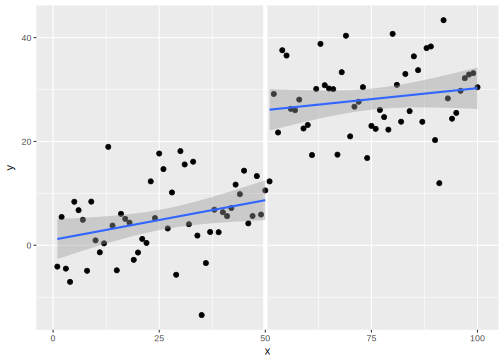
\includegraphics{pols503-notes_files/figure-latex/unnamed-chunk-2-1.pdf}

\hypertarget{refs}{}

\end{document}
